\section{Conjuntos e Lógica Fuzzy}
\subsection{Considerações iniciais}
Primeiramente introduzida em \cite{Zadeh1965}, onde o autor inicia a discussão definindo os
conjuntos fuzzy, sendo uma classe de objetos com valores contínuos de pertinência. Cada conjunto é
então caracterizado por uma função de pertinência, a qual atribui a cada objeto do conjunto um grau
de pertinência que varia entre zero e um. As operações matemáticas da teoria dos conjuntos, como
inclusão, união, intersecção, complemento, relação, etc., também são estendidas aos conjuntos fuzzy,
assim como várias propriedades dessas notações são definidas.

Uma das motivações da lógica fuzzy, vem da maneira como nosso cérebro classifica e rotula o mundo
real. Por exemplo, ao rotularmos uma pessoa como alta, estamos atribuindo ela ao grupo de pessoas
altas. Assim como quando nos expressamos sobre o quanto um determinado dia está fazendo calor ou
frio. O conjunto de pessoas altas ou dias frios, não se enquadra na sua totalidade na lógica
clássica. Pois essa forma imprecisa de descrever o mundo a nossa volta, desempenha um papel
fundamental na forma de pensar humana, assim como também nas áreas de reconhecimento de padrões,
comunicação e abstração\cite{Zadeh1965}.  Portanto esta seção tem como propósito contextualizar os
principais aspectos da lógica fuzzy que a torna tão importante no contexto da organização flexível
de documentos. Portanto definições mais aprofundadas sobre fuzzy fogem do escopo desse texto .
% TODO: Necessário informar o leitor sobre isso? Verificar com Tati

\subsection{Definição de conjuntos fuzzy}

Seja X um espaço de objetos, com um elemento genérico {\it x\/}.  Sendo $X= \big\{x\big\}$.
Um conjunto fuzzy $A$ em $X$ é caracterizado por uma função de pertinência $f_A(x)$, a qual associa
a cada elemento de $X$ um número real presente no intervalo de $[0,1]$, sendo o valor de $f_A(x)$ a
representação do grau de pertinência de $x$ em $A$.

\subsection{Lógica fuzzy}

A lógica fuzzy é uma lógica multi valorada, onde os valores das variáveis pertencem ao intervalo de
[0,1], enquanto na lógica clássica os valores verdades só possuem os estados 0 ou 1 (também
conhecido como valores {\it crisp\/}). Uma da mais importantes aplicações está no tratamento de
precisão e incerteza. O que nos permite a modelar soluções mais adequadas para ambientes imprecisos
e incertos.  Antes da lógica fuzzy ser introduzida em \cite{Zadeh1965}, em 1930
Lukasiewics\cite{Chen2000} desenvolveu a lógica n-valorada para $3 < n < \infty$, utilizando apenas
os operadores lógicos de negação $-$ e implicação $\Rightarrow$. Dado então um inteiro positivo, $n
> 3$, a lógica n-valorada assume valores verdade pertencente ao intervalo $[0,1]$, definidos pela
seguinte partição igualmente espaçada: $$0 =  \frac{0}{n-1},
\frac{1}{n-1},\frac{2}{n-1},...,\frac{n-2}{n-1},\frac{n-1}{n-1} = 1$$ Para estender a lógica
n-valorada para uma lógica com infinitos valores $2 \leq n \leq \infty$, \cite{Zadeh1965} modificou
a lógica de Lukasiewics definindo os seguintes operadores lógicos: $$\bar{a} = 1 -a$$ $$a \wedge b =
min\{a,b\}$$ $$a \vee b = max\{a,b\}$$ $$a \Rightarrow b = min\{1, 1+b-a\}$$ $$a \Leftrightarrow  b
= 1 - |a-b|$$

O objetivo da lógica fuzzy é prover mecanismos para tratar imprecisão e incerteza, se baseando na
teoria de conjuntos fuzzy e usando proposições imprecisas, de modo similar a lógica clássica usando
proposições precisas baseadas na teoria dos conjuntos.  Para entendermos essa noção, vejamos então
um mesmo exemplo pela ótica do raciocínio clássico e em seguida usando as ferramentas para descrever
imprecisão da lógica fuzzy.  \begin{enumerate}[label=\alph*)] \item Todo texto com 100 palavras ou
mais da área jurídica, tem como assunto o direito.  \item O texto A com título as manifestações
de junho, tem 100 palavras da área jurídica.  \item O texto B com título política nas
universidades, tem 99 palavras da área jurídica.  \item O texto A tem como assunto o direito e o
texto B não tem como assunto o direito.  \end{enumerate} Essa série de proposições ilustra o
raciocínio empregado na lógica clássica, e seguindo as regras de inferência conseguimos verificar
que as sentenças estão corretas. No entanto é fácil notar que a sentença d) não expressa muito bem o
nosso entendimento sobre a temática dos textos.  Seria comum alguém substituir a sentença d), por e)
O texto B fala um pouco sobre direito.  Vamos então adicionar a imprecisão comum no mundo real as
sentenças anteriores.  \begin{enumerate}[label=\alph*)] \item Todo texto que tem entre 50 e 100
palavras da área jurídica fala um pouco sobre direito.  Enquanto todo texto que contenha 100
ou mais palavras da área jurídica fala bastante sobre direito.  \item O texto A com título as
manifestações de junho, tem 100 palavras da área jurídica.  \item O texto B com título
política nas universidades, tem 99 palavras da área jurídica.  \item O texto A fala bastante
sobre direito, enquanto o texto B fala um pouco sobre direito.  \end{enumerate} Esse tipo de
dedução comumente utilizada no nosso dia a dia, não tem como ser tratada pela lógica
clássica. No entanto podemos lidar com esse tipo de inferência imprecisa, empregando a
lógica fuzzy, a qual permite o uso de alguns termos linguísticos imprecisos como:
\begin{itemize} \item Predicados fuzzy: antigo, raro, caro, alto, rápido \item Quantificadores
fuzzy: muito, pouco, quase, alguns \item Graus de verdade fuzzy: totalmente verdadeiro,
verdadeiro, parcialmente falso, falso, definitivamente falso \end{itemize}

%\section{Organização Flexível de Documentos}
%
%A organização de documentos tem sido uma área de fundamental importância no campo da mineração de
            %dados. Pois na era da informação, onde temos mídias sociais, internet das coisas e
            %computação móvel, produzindo diariamente uma elevada quantidade de dados estruturados e
            %não estruturados. 
%
%Se nos concentrarmos nos dados não estruturados, temos os dados textuais, que por sua vez pertencem
            %a uma ampla gama de tópicos que é constantemente atualizada, de maneira que a
            %organização deles em categorias não pode ser predefinida \cite{Carvalho2016}.  Diante
            %deste contexto, esse capítulo visa fundamentar as bases da organização flexível de
            %documentos seguindo o modelo defendido em \cite{Nogueira2013},


\section{Pré-Processamento} Pré-processamento dos dados é o processo de limpeza e preparação do
texto para classificação.  Assim como muitas palavras em um texto não causam nenhum impacto no
significado geral do documento\cite{Haddi2013}.  Soma se a isso o enorme custo computacional do
processo de mineração de textos, devido a grande quantidade de verbetes presente em dados textuais.
Portanto quanto maior for a coleção de textos, maior será a quantidade de palavras distintas.
Elevando bastante o custo computacional das tarefas de agrupamento e classificação, que por sua vez
são baseadas na análise do vocabulário dos documentos.  Com isso, vários pesquisadores propuseram
métodos para tentar simplificar, sintetizar e eliminar redundâncias desnecessárias nas coleções de
textos.  Pois, quanto mais compacto for a quantidade de verbetes da coleção de documentos, menor o
custo computacional e a quantidade de memória utilizada nas fases de agrupamento, extração de
descritores e classificação. A esse conjunto de técnicas realizadas inicialmente sobre os
documentos, denominamos de pré-processamento. 

A fase de pré-processamento voltada para a mineração de textos, requer técnicas muito diferentes no
preparo dos dados não estruturados para as fases posteriores, do que as técnicas comumente
encontradas nos métodos de descoberta de informação. As quais visam preparar dados estruturados para
as clássicas operações de mineração de dados \cite{Feldman2007}.

Segundo \cite{Feldman2007}, é possível categorizar de maneira clara as técnicas de pré-processamento
de textos em duas categorias, de acordo com as tarefas realizadas pela técnica e através dos
algoritmos e frameworks que a mesma utiliza. Por sua vez, as técnicas categorizadas pelas suas
tarefas, geralmente visam realizar a estruturação do documento através de tarefas e sub tarefas.
Como por exemplo, realizar a extração de título e sub título de documentos no formato PDF.  No
entanto, as demais técnicas de pré-processamento são derivadas de métodos formais, e incluem
esquemas de classificação, modelos probabilísticos e sistemas baseado em regras.

O processo de pré-processamento de dados textuais, inicia com um documento parcialmente estruturado
e avança incrementando a estrutura através do refinamento das características do documento e
adicionando novas \cite{Feldman2007}.  No contexto da mineração de textos as características dos
documentos são as suas palavras\cite{Haddi2013}. Ao final do processo, as palavras mais relevantes
são utilizadas, e as demais são descartadas. Uma vez que manter estas palavras torna a
dimensionalidade do problema maior, pois cada palavra no texto é tratada como uma
dimensão\cite{Haddi2013}.

O processo como um todo envolve várias etapas, as quais podemos elencar a remoção de espaços,
expansão de abreviações, remoção de $stopwords$, que são palavras que não possuem relevância no
significado geral do texto e geralmente são compostas por proposições, pronomes, artigos,
interjeições dentre outras\cite{Nogueira2013}. Assim como também o processo de $stemming$ ou
lematização, onde se busca encontrar o radical da palavra, visando assim remover palavras que
possuam significados similares. Ainda é possível usar as técnicas de NLP ($Natural Language
Processing$) para eliminar sinônimos. Por fim é realizada a seleção de termos \cite{Haddi2013}. 

Diversos métodos foram então propostos para se capturar a importância dos termos em coleções
textuais. Sendo o método { \it Term Frequency Inverse Document Frequency\/ }(TF-IDF) um dos mais
importantes\cite{Haddi2013} e frequentemente utilizado na literatura. A definição da TF-IDF está na
equação (\ref{eq:tfidf}), onde $N$ é o número de documentos da coleção, $DF$ o total de documentos
que possuem este termo e $FF$ ({\it frequency feature}) a frequência do termo no documento.

\begin{equation} \varphi(t,d) = FF * log(\frac{N}{DF}) \label{eq:tfidf} \end{equation}

Como resultado final de todo o processo de pré-processamento, obtém-se a matrix $D$. Onde $D$
representa os $n$ documentos da coleção, sendo cada documento $d_{i}$, com $1 \leq n \leq N$, uma
linha da matriz $D$, definido como sendo $ d_{i} =
[\varphi(t_{1},d_{i}),\varphi(t_{2},d_{i}),\varphi(t_{3},d_{i}),...,\varphi(t_{k},d_{i})] $, onde
$t_{j}$ é um termo presente na coleção, com $1 \leq j \leq k$.

\section{Agrupamento Fuzzy} O agrupamento é um processo não supervisionado \cite{Feldman2007}, onde
o objetivo é organizar os documentos similares no mesmo grupo e os documentos com grau de
dissimilaridade elevado em grupos distintos\cite{Nogueira2013}\cite{Feldman2007}. Este processo é de
grande utilidade para diversos campos de estudo da inteligência computacional, como a mineração de
dados, recuperação de informação, segmentação de imagens e classificação de padrões
\cite{Feldman2007}.

O problema de organizar os documentos de maneira a maximizar a similaridade entre os membros de um
mesmo grupo, e minimizar a similaridade entre documentos de grupos distintos, é essencialmente um
problema de otimização \cite{Feldman2007}.  Então pretende-se otimizar a escolha dos grupos, entre
todos as possibilidades de agrupamento, dada uma função objetivo que captura a qualidade dos grupos.
Esta função é responsável por atribuir ao conjunto de possíveis grupos um número real, de maneira
que quanto melhor for os grupos, maior será o seu valor\cite{Feldman2007}.

A medida de similaridade desempenha um papel fundamental no agrupamento, uma vez que ela precisa
expressar o quanto distante está um elemento do outro na coleção. Assim sendo, para obtermos bons
resultados durante a organização dos elementos é de grande importância a escolha adequada da medida
de similaridade, e esta escolha precisa ser feita de acordo com o tipo dos dados.  Na literatura a
medida de similaridade mais popular\cite{Feldman2007} é a distância euclidiana (Equação
\ref{eq:euclidiana}), que tem se mostrado bastante adequada em dados com baixa dimensionalidade.

\begin{equation} 
  D(x_{i}, x_{j}) = \sqrt{\sum_k{(x_{ik}-x_{jk})^2}} 
  \label{eq:euclidiana}
\end{equation}

No entanto, em coleções textuais a matriz documentos x termos é naturalmente esparsa, devido a
grande variedade de verbetes em uma coleção, o que faz com que um determinado documento $d_{i}$, não
contenha diversos termos presentes em um outro documento $d_{j}$. Resultando assim que o vetor de
características de cada documento, seja preenchido com vários zeros. Reduzindo então a eficácia da
distância euclidiana (Equação \ref{eq:euclidiana}) \cite{Nogueira2013}. Consequentemente a medida de
similaridade mais comum para coleções textuais é o coeficiente de similaridade de cosseno
\cite{Nogueira2013}\cite{Feldman2007}.  Por sua vez o coeficiente de similaridade de cosseno,
desconsidera os diversos zeros presentes nos vetores de termos dos documentos, levando em conta
apenas o ângulo formado entre eles\cite{Nogueira2013}.  Na equação (\ref{eq:simcos}) temos a
definição do coeficiente de similaridade de cosseno, onde $d_1$ e $d_2$, são dois documentos
quaisquer da coleção de documentos, e $1 \leq t \leq k$, onde $k$ é a quantidade total de termos da
coleção, e $d_{ik}$ a frequência do termo $t$ no documento $d_i$.

\begin{equation} 
  scos(d_{1}, d_{2}) = cos\theta = \frac{d_{1} \cdot d_{2}}{|d_{1}||d_{2}|} =
  \sum_{t=1}^k{\varphi(d_{1t},d_1) \cdot \varphi(d_{2t},d_2)} \in [0,1] 
  \label{eq:simcos}
\end{equation}

Os grupos resultantes desse processo, podem possuir algumas características que estão diretamente
relacionadas com o método de agrupamento empregado. Estes podem ser $hard$ ou $crisp$, caso o método
de agrupamento seja baseado na lógica clássica, assim como podem ser $soft$, caso o método seja
baseado na lógica fuzzy. No agrupamento $hard$, cada documento $d_{i}$ só poderá pertencer a um
único grupo $g_{j}$ \cite{Bezdek1984}. Enquanto em grupos $soft$, cada documento $d_{i}$ pode
pertencer a um ou mais grupos $g_{j}$, com grau de pertinência variados.  Além destes, os grupos
ainda podem ser $flat$ ou hierárquicos, onde no agrupamento $flat$ todos os grupos estão no mesmo
nível, enquanto no modelo hierárquico os grupos podem estar dispostos em uma hierarquia, de modo que
uma relação de parentesco é definida entre eles.

Portanto, seja $G = \{g_{1},g_{2},g_{3},...,g_{c}\}$ os grupos resultantes do agrupamento, sendo $c$
o total de grupos. No agrupamento $hard$, a pertinência de cada documento $d_{i}$ pode ser
representada pela função de pertinência $\kappa(d_{i}, g_{j}) \in \{0,1\}$, tal que $\sum_{j=1}^c
\kappa(d_{i}, g_{j}) = 1$.  Um dos mais populares algoritmos a implementar essa abordagem $hard$ é o
K Means.  Em \cite{Bezdek1984}\cite{Nogueira2013}\cite{Feldman2007}, é apontado uma falha inerente
dessa abordagem, pois quando um documento só pode pertencer a um único grupo, fica evidenciado que o
mesmo não compartilha nenhuma similaridade com os documentos dos demais grupos, o que não expressa a
imprecisão intrínseca da sobreposição dos assuntos em documentos de texto.

Com o objetivo de tratar essa falha da abordagem $hard$ e adicionar o tratamento de imprecisão e
incerteza no agrupamento, \cite{Bezdek1984} utilizou o modelo de partições fuzzy definido em
\cite{Zadeh1965}, para permitir pertinências parciais de um elemento a um grupo, propondo assim o
algoritmo Fuzzy C Means (FCM).  Sendo assim, a função de pertinência de um documento $d_{i}$ em um
grupo $g_{j}$, pode ser definida como sendo $\mu(d_{i}, g_{j}) \in [0,1]$, tal que $\sum_{j=1}^m
\mu(d_{i}, g_{j}) = 1$.

Outro desafio sempre presente em métodos de agrupamento é a descoberta do número ideal de grupos em
uma coleção. O método de organização flexível proposto em \cite{Nogueira2013} utiliza a  $Fuzzy\
Silhouette$ (FS) para realizar a validação do agrupamento fuzzy, e por conseguinte encontrar o
número de grupos ideal. A função FS é uma adaptação do método de critério de largura média
($Average\ Silhuette\ Width\ Criterion$ - ASWC), desenvolvido para o agrupamento $crisp$
\cite{Nogueira2013}. A definição da silhueta fuzzy está nas equações (\ref{eq:silhuette}) e
(\ref{eq:fs}), onde $\alpha(d_i, g_l)$ é a distância média entre o documento $d_i$ e todos os
documentos presentes no grupo $g_l$, enquanto $\beta(d_i,g_l) = min\{\alpha(d_i,g_h) | 1 \leq h \leq
c; h \neq l\}$, é a medida de dissimilaridade de $d_i$ ao grupo vizinho mais próximo de $g_l$, tal
que $c$ é a quantidade de grupos.  \begin{equation} S(d_i) = \frac{\beta(d_i, g_l) -
\alpha(d_i,g_l)}{max\{\alpha(d_i,g_l), \beta(d_i,g_l)\}} \label{eq:silhuette} \end{equation}
\begin{equation} FS = \frac{\sum_{i=1}^n{(\mu_1(d_i) - \mu_2(d_i))}S(d_i)}{\sum_{i=1}^n{(\mu_1(d_i)
  - \mu_2(d_i))}} \label{eq:fs} \end{equation} Na equação (\ref{eq:fs}), $\mu_1(d_i)$ é maior
  pertinência do documento $d_i$ em um grupo, enquanto $\mu_2(d_i)$ é a segunda maior. Quanto maior
  então for o valor da função FS, melhor será o agrupamento. Deste modo para encontrar o número de
  grupos ideal, basta executar a função FS variando o número de grupos, e selecionar o agrupamento
  que tiver o valor máximo de FS.

Toda investigação realizada neste trabalho tomou como base os métodos de agrupamento que derivam do
algoritmo FCM\cite{Bezdek1984}, para se beneficiar da capacidade de tratar imprecisão e incerteza da
lógica fuzzy, e por conseguinte permitir que um mesmo documento seja categorizado em mais de um
tópico, refletindo a realidade dos documentos textuais. Utilizando como medida de similaridade o
coeficiente de similaridade de cosseno (Equação \ref{eq:simcos}). E por fim a quantidade de grupos
ideal foi escolhida utilizando o método da silhueta fuzzy ( Equação \ref{eq:fs}).

\subsection{Algoritmo Fuzzy C Means (FCM)} \cite{Bezdek1984} descreve um método de agrupamento fuzzy
que produz como saída partições fuzzy e protótipos dos grupos. Esse algoritmo desempenha um papel
importante no contexto do agrupamento fuzzy, devido seu pioneirismo no campo de estudo, possuindo
diversas extensões. Assim como também é considerado um dos mais amplamente utilizados métodos de
agrupamento fuzzy da literatura\cite{Pal2005}. Sendo a maioria dos métodos de agrupamento fuzzy,
derivações do FCM\cite{Krishnapuram1993}.

Seja então $V = \{v_1,v_2,v_3,...,v_c\}$ os protótipos dos grupos $G = \{g_1,g_2,g_3,...g_c\}$
definidos por 
\begin{equation} 
  V = \left\{ v_j | v_j = \frac{\sum_{i=1}^n[\mu(d_i,g_j)]^m d_i}{\sum_{i=1}^n[\mu(d_i,g_j)]^m}, 
  1 < j \leq c \right\} 
  \label{eq:prototipos} 
\end{equation}
, tal
que $v_i$ seja o protótipo de $g_i$, $c$ o número de grupos gerados no agrupamento e $n$ o número de
documentos presentes na coleção. Bem como seja 
\begin{equation} 
  U_{c \times n} = \{\mu(d_i, g_k) |\mu(d_i, g_k) \in [0,1], 1 < i \leq n, 1 < k \leq c, eqs
  (\ref{eq:fcmrestri1})(\ref{eq:fcmrestri2})\} 
  \label{eq:part_fuzzy} 
\end{equation} 
uma partição fuzzy, com todas as pertinências dos documentos aos grupos. Sendo $m$ o fator de
fuzificação, que regula o quão fuzzy será as partições finais. De modo que para $m = 1$ a partição
resultante é totalmente $crisp$ (figura \ref{fig:cluster_crisp}) e para $m \rightarrow \infty$ a
interseção entre os grupos tende a aumentar (figura
\ref{fig:cluster_fuzzy})\cite{Pal2005}\cite{Nogueira2013}. Segundo \cite{Bezdek1984} nenhuma teoria
ou evidência computacional aponta para um valor ótimo de $m$, contudo o autor aponta que a faixa de
valores ideais aparenta ser [1,30]. Sendo assim, se existir um conjunto de dados para teste, uma boa
estratégia para a escolha de $m$ é a realização de testes experimentais. Caso contrário, o intervalo
de [1.5, 3.0] aparenta trazer bons resultados para a maior parte dos dados.

\begin{figure}[!htp] \centering 
  \begin{minipage}{0.45\textwidth} 
    \centering
    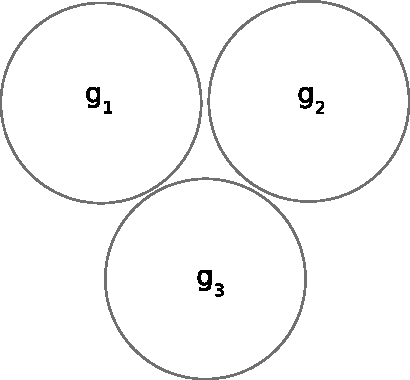
\includegraphics[width=0.6\columnwidth]{assets/clusters_crisp.pdf} 
    \caption{Ilustração denotando os
grupos $g_1,g_2,g_3$ organizados sem sobreposição, para $m = 1$.} \label{fig:cluster_crisp}
  \end{minipage}\hfill 
  \begin{minipage}{0.45\textwidth} \centering
    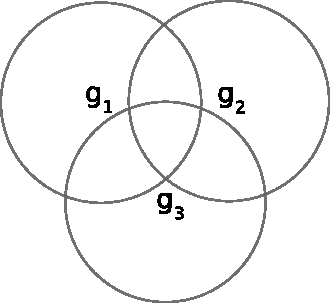
\includegraphics[width=0.6\columnwidth]{assets/clusters_fuzzy.pdf} 
    \caption{Ilustração denotando os
    grupos $g_1,g_2,g_3$ organizados de maneira fuzzy, com sobreposição, quando 
    $m \rightarrow \infty$.}
    \label{fig:cluster_fuzzy} 
  \end{minipage} 
\end{figure} 
E ademais a função de pertinência
$\mu(d_i,g_k)$ de cada documento na coleção, é definida como sendo 
\begin{equation} 
  \mu(d_i,g_k) = \frac{1}{\sum_{j=1}^n(\frac{dist(d_i,v_k)}{dist(d_i,v_j)})^{\frac{1}{m-1}}} 
  \label{eq:pertinencia}
\end{equation}
, tal que $\mu(d_i, g_k)$ está sujeita as equações \begin{equation} \sum_{k=1}^c
\mu(d_i,g_k) = 1 \label{eq:fcmrestri1} \end{equation} e \begin{equation} 0 < \sum_{i=1}^n
\mu(d_i,g_k) < n \label{eq:fcmrestri2} \end{equation} . Onde usualmente no contexto do
agrupamento de coleções textuais $dist(d_i,g_k) = scos(d_i,g_k)$.  Sendo assim a restrição
(\ref{eq:fcmrestri2}) da equação (\ref{eq:pertinencia}) tem como função evitar que algoritmo
FCM produza grupos vazios\cite{Nogueira2013}. Enquanto a equação (\ref{eq:fcmrestri1}) impõe
que a soma das pertinências seja sempre igual a um.  Entretanto a restrição
(\ref{eq:fcmrestri2}) produz um problema em elementos equidistantes aos grupos. Ou seja,
quando temos o caso $\mu(d_i, g_1) = \mu(d_i, g_2) = ... = \mu(d_i, g_c)$. Nessa situação o grau de
pertinência do elemento a cada grupo será a pertinência média, ou seja $\mu(d_i, g_1) = \mu(d_i,
g_2) = ... = \mu(d_i, g_c) = \frac{1}{c}$. Supondo agora um segundo documento $d_2$, que seja mais
distante do que $d_1$, porém assim como $d_2$, também equidistante aos grupos, temos que $\mu(d_2,
g_j) = \mu(d_1, g_j) = \frac{1}{c}$, para $1 < j \leq c$. Nesse contexto a pertinência de $d_2$ e
$d_1$, não expressa a distância relativa desses documentos aos grupos. Esse problema está ilustrado
na Figura (\ref{fig:fcm_problem}).

\begin{figure}[!htp] \centering
  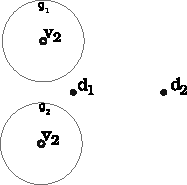
\includegraphics[width=0.4\columnwidth]{assets/clusters_fcm_problem.pdf} 
  \caption{Problema dos
    elementos equidistantes do algoritmo FCM. Na imagem $g_1$ e $g_2$ são grupos, com os seus
    respectivos protótipos $v_1$ e $v_2$. Enquanto $d_1$ e $d_2$ são documentos equidistantes aos
    protótipos $v_1$ e $v_2$. Portanto $\mu(d_1,g_1) = \mu(d_1,g_2) = \mu(d_2,g_1) = \mu(d_2,g_2) =
0.5$.} 
  \label{fig:fcm_problem} 
\end{figure}

Segundo \cite{Bezdek1984} várias funções de otimização das partições fuzzy produzidas no agrupamento
foram propostas. Sendo a minimização da função objetivo $J(U_{c \times n},G,V,D)$, que visa
minimizar a distância entre os documentos e os protótipos dos grupos\cite{Nogueira2013}, definida na
equação (\ref{eq:fcm_obj}) a mais popular.  \begin{equation} min\{(J(U_{c \times n},G,V,D) =
\sum_{i=1}^n \sum_{j=1}^c [\mu(d_i, g_j)]^m dist(d_i, v_j)\} \label{eq:fcm_obj} \end{equation} O
mais utilizado algoritmo para soluções aproximadas da minimização (\ref{eq:fcm_obj}), é a iteração
de Picard\footnote{Método iterativo para construção de soluções aproximadas, atribuído ao matemático
francês Charles Emile Picard (1856-1941).
\url{http://mathfaculty.fullerton.edu/mathews/n2003/PicardIterationMod.html}}\cite{Pal2005} através
das equações (\ref{eq:prototipos})(\ref{eq:part_fuzzy}). Sendo assim  o ciclo de aproximações se dá
por $V_{t-1} \Rightarrow  U_t \Rightarrow  V_t$, onde ao final de cada iteração é verificado se
$\parallel V_{t-1} - V_t\parallel < \varepsilon$.  A literatura também expressa que os ciclos podem
começar pela partição fuzzy, fazendo então $U_{t-1} \Rightarrow  V_t \Rightarrow  U_t$, e ao final
do ciclo checando o erro mínimo com $\parallel U_{t-1} - U_t\parallel < \varepsilon$, sendo $t$ o
contador de iterações.  Contudo existem benefícios em termos de processamento e memória ao utilizar
a iteração iniciando e finalizando com $V$\cite{Pal2005}.  \cite{Bezdek1984} e \cite{Pal2005}
afirmam que a convergência desse modelo iterativo ocorre em ambos os tipos de ciclo.  A partição
fuzzy inicial $U_0$ é comumente inicializada com valores aleatórios\cite{Nogueira2013} ou com o
resultado de um agrupamento previamente executado\cite{Pal2005}\cite{Krishnapuram1993}. Nas demais
iterações a atualização dos protótipos é realizada a partir da equação (\ref{eq:prototipos}). O
pseudo código utilizando essa abordagem iterativa está listado no algoritmo (\ref{alg:fcm}), no qual
$\textbf{{\color{blue}inicializa-particao-fuzzy}(D,G)}$, pode ser uma das duas formas de
inicialização descritas anteriormente.

\begin{algorithm}[H] 
  \SetAlgoLined \KwData{D, c, m, $\varepsilon$} 
  \KwResult{V, U} 
  G $\gets$ $[g_1,g_2,...,g_c]$\; 
  $U_0$ $\gets$ \textbf{{\color{blue}inicializa-particao-fuzzy}(D,G)}\; 
  $t \gets 0$\; 
  \Do{ $\parallel U_{t-1} - U_t\parallel > \varepsilon$ }{ 
    $V_t$ $\gets$ calcula usando (\ref{eq:prototipos})\; 
    $t \gets t + 1$\; 
    $U_t$ $\gets$ calcula usando (\ref{eq:part_fuzzy})\; 
  }
  $\textbf{retorne} (U_t, V_t)$\; 
  \caption{Pseudo código da implementação iterativa do método FCM}
\label{alg:fcm} \end{algorithm}

Por fim está ilustrado na figura (\ref{fig:samples_fcm}), os resultados produzido pelo algoritmo
FCM, em dois conjuntos de coordenadas no $R^2$. Na figura os pontos foram pintados com a cor
correspondente ao grupo em que o mesmo obteve o maior valor de pertinência.

\begin{figure}[!htp] 
  \centering 
  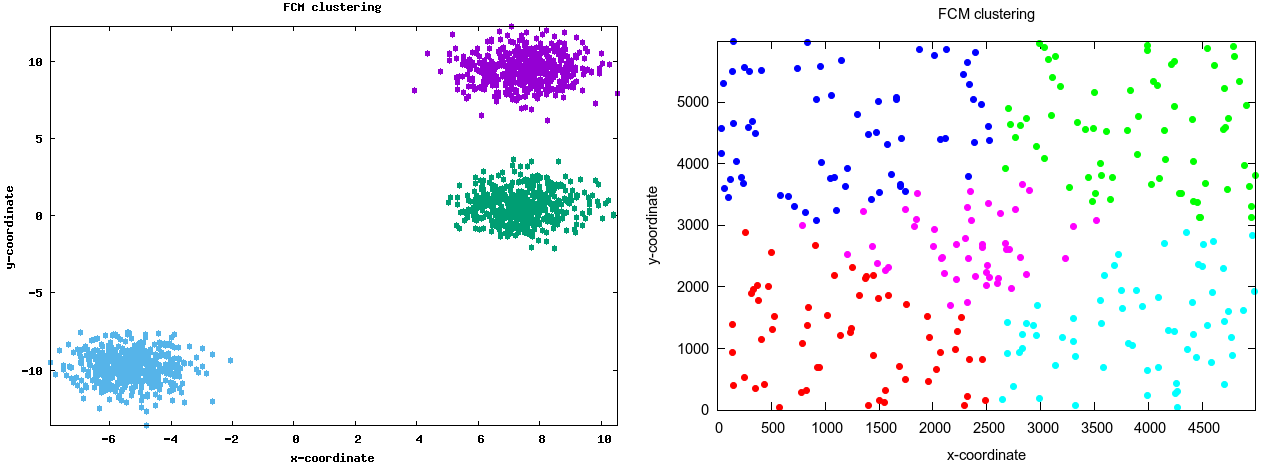
\includegraphics[width=0.8\columnwidth]{assets/samples_fcm.png}
  \caption{Resultado do agrupamento de dois conjuntos de coordenadas no $R^2$ usando o algoritmo
  FCM\protect\footnotemark.} 
  \label{fig:samples_fcm} 
\end{figure}

\subsection{Algoritmo Possibilistic C Means (PCM)}

A restrição probabilística (\ref{eq:fcmrestri2}) do FCM que obriga a soma das pertinências de
um elemento ser igual a um, nem sempre resulta em pertinências que representam bem a realidade dos
dados, conforme exemplificado na figura (\ref{fig:fcm_problem}).  Esse problema se agrava ainda
mais, em bases com muitos dados ruidosos ($outliers$).  Visando então contornar esses problemas do
FCM, foi proposto em \cite{Krishnapuram1993} o algoritmo $Possiblistic\ C\ Means$ (PCM). 

Ao contrário do FCM, o PCM não atribui pertinências dos documentos aos grupos, e sim tipicidades. 
Que podem ser interpretadas como graus de possibilidade de um elemento pertencer ao grupo. Como
consequência a partição resultante é possibilística. Para se adequar a essa abordagem
possibilística, a função objetivo do PCM deriva da equação (\ref{eq:fcm_obj}) do FCM. Tendo também 
as funções de atualização de prótotipos e atribuição de pertinências modificadas.

Na teoria de conjuntos fuzzy, a pertinência de um elemento a um grupo fuzzy não depende da
pertinência desse mesmo elemento em outro grupo. No entanto no modelo FCM, a restrição
(\ref{eq:fcmrestri2}) torna dependente a pertinência dos elementos aos grupos. De maneira que
se um elemento obtiver um grau elevado de pertinência em um dado grupo, ele não poderá ter uma
pertinência também elevada em outro grupo, ou seja $\mu(d_1, g_1) = 1-\mu(d_1,g_2)$, supondo um
agrupamento com dois grupos. Portanto \cite{Krishnapuram1993} relaxa a restrição
(\ref{eq:fcmrestri2}), fazendo com que a pertinência dependa unicamente da distância do
elemento ao grupo. Logo as restrições (\ref{eq:fcmrestri1}) e (\ref{eq:fcmrestri2}), são 
redefinidas nas equações (\ref{eq:pcmrestri1})(\ref{eq:pcmrestri2}), onde $\lambda(d_i,g_j)$
representa a tipicidade do documento $d_i$ em relação ao grupo $g_j$.
\begin{equation}
  \lambda(d_i, g_j) \in [0,1], \forall i,j
  \label{eq:pcmrestri1}
\end{equation}

\begin{equation}
  0 < \sum_{j=1}^n \lambda(d_i, g_j) \leq n, \forall j
  \label{eq:pcmrestri2}
\end{equation}
Após relaxar a restrição (\ref{eq:fcmrestri2}) se mantivermos a função objetivo do FCM 
(equação \ref{eq:fcm_obj}), teríamos uma solução trivial, bastando atribuir $0$ a todas as
pertinências para minimizar $J(U_{c \times n},G,V,D)$\cite{Krishnapuram1993}\cite{Nogueira2013}. 
Portanto buscando evitar essa solução trivial, e 
manter a característica de atribuir aos elementos representativos pertinências elevadas aos grupos e 
penalizar os elementos não representativos, a função objetivo é reformulada como sendo 
\begin{equation}
  K_m(P_{c \times n},G,V,D) = \sum_{j=1}^c \sum_{i=1}^n [\lambda(d_i, g_j)]^m dist(d_i, v_j) +
  \sum_{j=1}^c \gamma_j \sum_{i=1}^n [1 - \lambda(d_i, g_j)]^m
  \label{eq:pcmobj}
\end{equation}
, onde $\gamma_j > 0$ são parâmetros que determinam a distância a qual o valor de pertinência
(tipicidade) se torna $0.5$. \cite{Krishnapuram1993} explica que $\gamma_j$ seja escolhido
a depender da faixa de possibilidades (pertinência) desejada para um grupo. Por exemplo, 
$\gamma_j$ pode ser igual para todos os grupos, quando se deseja que a forma dos grupos seja similar.
Contudo na maioria dos casos se espera que $\gamma_j$ reflita o formato e tamanho particular de cada
grupo. Assim sendo, o autor indica que a definição (\ref{eq:pcmgamma}) se mostra adequada para maior
parte dos dados, onde $L$ é usualmente 1.
\begin{equation}
  \gamma_j = L \frac{\sum_{i=1}^n \lambda(d_i,g_j)^m dist(d_i,v_j)}{\sum_{i=1}^n \lambda(d_i,g_j)^m}
  \label{eq:pcmgamma}
\end{equation}
A partição de pertinências possibilísticas produzidas pelo PCM é então definida como sendo
\begin{equation} 
  P_{c \times n} = \{\lambda(d_i, g_k) |\lambda(d_i, g_k) \in [0,1], 1 < i \leq n, 1 < k \leq c, eqs
  (\ref{eq:pcmrestri1})(\ref{eq:pcmrestri2})\}
  \label{eq:pcmpart} 
\end{equation} 
\begin{equation}
  \lambda(d_i,g_j) = \frac{1}{1+\left(\frac{dist(d_i,g_j)}{\gamma_j}\right)^{\frac{1}{m-1}}}
  \label{eq:lambda}
\end{equation}
, enquanto a atualização de protótipos ocorre de maneira similar a equação (\ref{eq:prototipos}) do
FCM, apenas alterando a pertinência $\mu(d_i,g_j)$ por $\lambda(d_i,g_j)$. A síntese do 
algoritmo PCM está apresentada em forma de pseudo código no algoritmo (\ref{alg:pcm}). 

\begin{algorithm}[H] 
  \SetAlgoLined \KwData{D, c, m, $\varepsilon$} 
  \KwResult{V, P} 
  G $\gets$ $[g_1,g_2,...,g_c]$\; 
  $P_0$ $\gets$ \textbf{{\color{blue}inicializa-particao-fuzzy}(D,G)}\; 
  $\gamma_j \gets$ calcula utilizando (\ref{eq:pcmgamma})\;
  $t \gets 0$\; 
  \Do{ $\parallel P_{t-1} - P_t\parallel > \varepsilon$ }{ 
    $V_t$ $\gets$ calcula usando (\ref{eq:prototipos})\; 
    $t \gets t + 1$\; 
    $P_t$ $\gets$ calcula usando (\ref{eq:pcmpart})\; 
  }
  $\textbf{retorne} (P_t, V_t)$\; 
  \caption{Pseudo código da implementação iterativa do método PCM}
  \label{alg:pcm} 
\end{algorithm}
Por fim está ilustrado na figura (\ref{fig:samples_pcm_fcm}) (a), o resultado do agrupamento
obtido pelo método FCM, e em (b) o agrupamento gerado pelo algoritmo PCM em um conjunto de 
coordenadas no $R^2$. Na figura os pontos foram pintados com a cor correspondente ao grupo em que o 
mesmo obteve o maior valor de pertinência. Observa-se nessa comparação simplificada que o algoritmo 
PCM tentou maximizar a pertinência dos pontos aos grupos maiores, ocasionando uma maior quantidade
de pontos com pertinência elevada em dois grupos, ao contrário do FCM que distribuiu de maneira
uniforme os pontos em 4 grupos.

\begin{figure}[!htp] 
  \centering 
  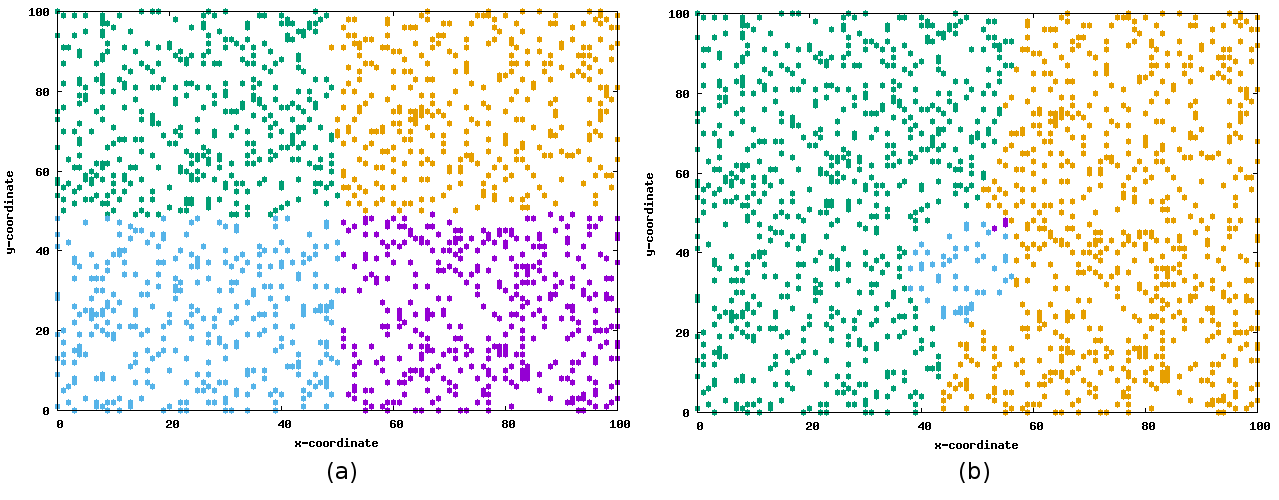
\includegraphics[width=0.8\columnwidth]{assets/samples_pcm_fcm.png}
  \caption{Demonstração de agrupamentos obtidos com os algoritmos 
    FCM\protect\footnotemark (a) e PCM\protect\footnotemark[\value{footnote}](b)
  .} 
  \label{fig:samples_pcm_fcm} 
\end{figure}

\subsection{Algoritmo Possibilistic Fuzzy C Means (PFCM)} 
De acordo com \cite{Pal2005} o algoritmo PCM pode levar os resultados do agrupamento 
a conter grupos coincidentes, ou seja quando o protótipo $v_i$ está muito próximo de outro protótipo
$v_j$. Segundo os autores, isto ocorre quando a inicialização da partição inicial não possui 
protótipos
suficientemente separados. Esse problema não é causado por uma escolha ruim da penalidade presente
na função objetivo do PCM, o que ocorre é uma falta de restrições para evitar que isso aconteça.

\cite{Carvalho2016} cita que as pertinências do FCM e as tipicidades do PCM são ambas importantes
para a correta interpretação das sub estruturas dos dados. Pois quando se tem dados que precisam
ser rotulados de maneira $hard$, as pertinências se mostram como uma escolha adequada, de modo que é
intuitivo atribuir o elemento ao grupo em que o mesmo possua a menor distância. Por outro lado,
durante a atualização dos protótipos, as tipicidades desempenham um papel fundamental para 
aliviar os efeitos indesejados dos dados ruidosos.

Com o propósito de aproveitar então os benefícios de ambas as abordagens, \cite{Pal2005} propôs o
algoritmo PFCM, que utiliza as pertinências $\mu(d_i,g_j)$ do FCM e as tipicidades
$\lambda(d_i,g_j)$ do PCM. Deixando o usuário definir a proporção de cada uma das contribuições com
parâmetros que ponderam o peso de ambos. Portanto é realizado uma mistura entre as funções objetivo
(\ref{eq:fcm_obj}) e (\ref{eq:pcmobj}) resultando na minimização da função objetivo
(\ref{eq:pfcmobj}), que está sujeita as condições de (\ref{eq:pfcmrestri}), onde 
$a,b > 0$ e $m,n > 1$. Os parâmetros $a,b$ representam a importância
relativa dos valores de pertinência e tipicidades e devem ser definidos pelo usuário de acordo com o
problema. Os autores sugerem que $b$ seja maior que $a$, porém não muito maior, para não eliminar
completamente os benefícios do FCM. 
\begin{equation}
  L_m(U_{c \times n},P_{c \times n},G,V,D) = \sum_{j=1}^c 
  \sum_{i=1}^n [a\mu(d_i,g_j)^n + b\lambda(d_i, g_j)^m] dist(d_i, v_j) +
  \sum_{j=1}^c \gamma_j \sum_{i=1}^n [1 - \lambda(d_i, g_j)]^m
  \label{eq:pfcmobj}
\end{equation}
\begin{equation}
  \sum_{j=i}^c \mu(d_i,g_j) = 1, \forall i, 0 < \mu(d_i,g_j),\lambda(d_i,g_j) \leq 1
  \label{eq:pfcmrestri}
\end{equation}
A mistura e as ponderações adicionados no algoritmo PFCM também são agregadas a função de
atualização dos protótipos (\ref{eq:pfcmproto}), a qual passa a se beneficiar das características de
ambos os algoritmos.
De maneira a reduzir os efeitos dos dados ruidosos, minimizar o problema dos protótipos coincidentes
e evitar a singularidade do FCM. O pseudo código do PFCM é apresentado no Algoritmo \ref{alg:pfcm}, 
onde a
função $\textbf{\color{blue}inicializa-prototipos}(D,G)$ gera os protótipos iniciais da partição
$V_0$. Como resultado demonstrativo desse algoritmo está ilustrado na figura
(\ref{fig:samples_pfcm}), onde é possível observar que os grupos produzidos são em certa perspectiva
um intermédio entre o agrupamento produzido pelo FCM e PCM no mesmo conjunto de dados, apresentados
na figura (\ref{fig:samples_pcm_fcm}).
\begin{equation}
  V = \left\{ v_j | v_j = \frac{\sum_{i=1}^n[a\mu(d_i,g_j)^n + b\lambda(d_i, g_j)^m] d_i}
    {\sum_{i=1}^n[a\mu(d_i,g_j)^n + b\lambda(d_i, g_j)^m]}, 
  1 < j \leq c \right\} 
  \label{eq:pfcmproto}
\end{equation}

\begin{algorithm}[H] 
  \SetAlgoLined \KwData{D, c, m, $\varepsilon$} 
  \KwResult{V, P} 
  G $\gets$ $[g_1,g_2,...,g_c]$\; 
  $V_0$ $\gets$ \textbf{{\color{blue}inicializa-prototipos}(D,G)}\; 
  $\gamma_j \gets$ calcula utilizando (\ref{eq:pcmgamma})\;
  $t \gets 0$\; 
  \Do{ $\parallel V_{t-1} - V_t\parallel > \varepsilon$ }{ 
    $U_t$ $\gets$ calcula com (\ref{eq:part_fuzzy}) usando $V_{t-1}$\; 
    $P_t$ $\gets$ calcula com (\ref{eq:pcmpart}) usando $V_{t-1}$\; 
    $V_t$ $\gets$ calcula com (\ref{eq:pfcmproto})\; 
    $t \gets t + 1$\; 
  }
  $\textbf{retorne} (U_t,P_t,V_t)$\; 
  \caption{Pseudo código da implementação iterativa do método PFCM}
  \label{alg:pfcm} 
\end{algorithm}

\begin{figure}[!htp] 
  \centering 
  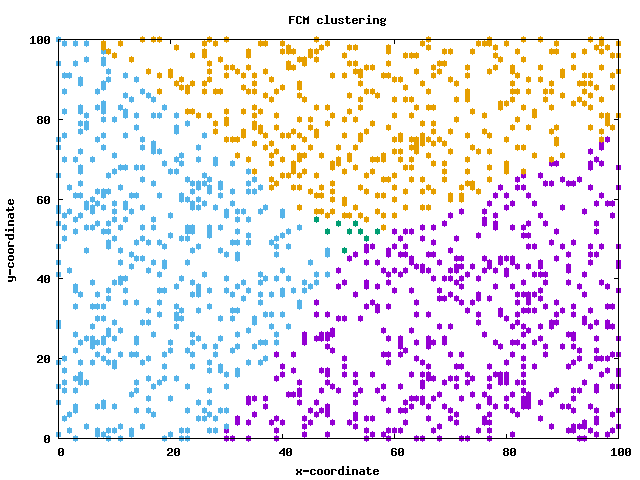
\includegraphics[width=0.6\columnwidth]{assets/samples_pfcm.png}
  \caption{Demonstração do agrupamento obtido com os algoritmo 
    PFCM\protect\footnotemark em um conjunto de coordenadas de pontos no $R^2$.} 
  \label{fig:samples_pfcm} 
\end{figure}

\subsection{Algoritmo Hierarchic Fuzzy C Means (HFCM)}
Documentos de texto tratam de vários temas, como política, esporte, tecnologia e etc.
E os métodos de agrupamento $soft$, como FCM e PCM, quando aplicados a coleções textuais, buscam
encontrar semelhanças entre os documentos e agrupar por tópicos. Porém acontece, que um
tópico pode se dividir em sub temas, como por exemplo esporte, que pode se dividir em futebol,
vôlei, tênis e etc. Deste modo os temas presentes em uma coleção textual podem ser organizados 
em uma hierarquia de tópicos conforme a figura \ref{fig:hierarquia}. Portanto construir hierarquias
utilizando métodos de agrupamento fuzzy é o propósito principal do algoritmo HFCM proposto em
\cite{PedryczR2006}.

\begin{figure}[!htp] 
  \centering 
  \Tree [.Documentos [.Esporte [.Futebol ] [.Vôlei ] [.Karatê ] ] [.Ciência [.Biologia ] 
  [.Física ] [.Química ] [.Astronomia ]] ]
  \caption{Exemplo de hierarquia de tópicos presentes em uma coleção de textos.}
  \label{fig:hierarquia}
\end{figure}

O HFCM consegue realizar essa tarefa, expandindo sucessivamente as folhas presentes na hierarquia em
subgrupos mais detalhados\cite{PedryczR2006}. Onde a expansão é realizada através de novos
agrupamentos com o algoritmo CFCM, que é uma versão condicional do FCM. No entanto o primeiro nível
da hierarquia é o resultado direto do algoritmo FCM, enquanto os demais níveis são agrupamentos
obtidos com o CFCM, sobre a coleção de documentos filtrada grupo a ser expandido. 

Seja então $D = \{d_1,d_2,...,d_n\}$ um conjunto com $n$ documentos, então o HFCM executa sobre $D$
o algoritmo FCM produzindo o primeiro nível da hierarquia o método. Como resultado é gerada uma 
partição fuzzy $U_{c \times n}[1]$ e os protótipos 
$V[1] = \{v_1[1],v_2[1],...,v_c[1]\}$, onde $[1]$ representa o nível da 
hierarquia.

A expansão ocorre sempre nas folhas da hierarquia, e a decisão de expandir um determinado grupo, 
se dá pela avaliação do
agrupamento, que é realizado através do índice de desempenho $Q$ (\ref{eq:qindex1})(\ref{eq:qindex2})
, onde $Q$ representa a qualidade dos protótipos gerados pelo agrupamento. De maneira que quanto 
melhor for um 
grupo mais próximo de zero
será o resultado da medida de desempenho $Q$, e quanto maior for o desempenho pior será o
grupo. Portanto o grupo que obtiver o maior valor de $Q$, será escolhido para a
expansão condicional através do CFCM. Considere então $j$ o grupo com maior valor de $Q$ do nível
$l$ da hierarquia e
\begin{equation}
  D_j[l] = \left\{d_{k} | \mu(d_{k}, g_j[l]) \leq \frac{1/l}{c}\right\}
  \label{eq:cfcmfilter}
\end{equation}
a coleção de documentos selecionados do grupo $j$ com
pertinência maior que a pertinência média. O agrupamento com o algoritmo CFCM é então executado
sobre a coleção $D_j[l]$ produzindo $c$ novos grupos para o nível $l+1$ da hierarquia. Todo o
processo se repete então para o nível $l+1$ da hierarquia, e assim sucessivamente. Segundo os
autores o ponto de parada da expansão hierárquica pode ser uma profundidade predefinida pelo usuário
, com a estabilização das medidas de desempenho dos grupos ou supervisionada, de modo que o usuário
observa a hierarquia que está sendo produzida e interrompe o processo quando
desejar\cite{PedryczR2006}.

\begin{equation}
  Q_j[1] = \sum_{d_i \in g_j} dist(d'_i,d_i)^2
  \label{eq:qindex1}
\end{equation}
\begin{equation}
  Q'_j[2] = \sum_{d_i \in g_j} dist(d'_i,d_i)^2
  \label{eq:qindex2}
\end{equation}
\begin{equation}
  d'_i = \sum_{h=1}^c \mu(d_i,g_h)[1]v_h[1] 
  \label{eq:dlinha1}
\end{equation}
\begin{equation}
  d'_i = \sum_{h=1}^c \mu'(d_i,g_h)[j,2]v_h[2] 
  \label{eq:dlinha2}
\end{equation}

Segundo \cite{Nogueira2013},
os protótipos dos grupos representam uma versão condensada dos documentos agrupados, portanto
$d_i$ também pode ser representado pela combinação linear das pertinências de $d_i$ com os
protótipos, resultando em $d'_i$. Logo é esperado que $d'_i$ seja o mais próximo possível do 
documento
original $d_i$. Consequentemente, é utilizado essa noção para estimar a qualidade de um grupo
através das equações \ref{eq:qindex1} para o nível inicial da hierarquia e \ref{eq:qindex2} nos
demais níveis, onde $Q$ calcula a soma total das distâncias dos documentos $d_i$ de um grupo com
$d'_j$.

A atualização dos protótipos no algoritmo CFCM ocorre da mesma maneira que o a equação
(\ref{eq:prototipos}) do FCM, contudo a função de pertinência é redefinida como sendo
\begin{equation}
  \mu(d_i,g_h[l]) = \frac{\mu(d_i,g_j[l-1])}
  {\sum_{k=1}^c \left(\frac{dist(d_i,v_h[l])}{dist(d_i,v_k[l])}\right)^{\frac{1}{m-1}}}, 
  1 < h \leq c,
  d_i \in D_j[l-1], eq (\ref{eq:cfcmrestri1})
  \label{eq:pertcfcm}
\end{equation}
, cujo o valor de $l$ corresponde ao nível da hierarquia e $g_j$ seja o grupo 
expandido no nível $l-1$.
Portanto percebe-se que a pertinência
de um documento $d_i$ em um grupo $g_h[l]$, será no máximo a pertinência do documento ao grupo que
foi expandido. Com isso temos a restrição \ref{eq:fcmrestri2} do FCM adaptada no CFCM para
\begin{equation}
  \sum_{h=1}^c \mu(d_i,g_h[l]) = \mu(d_i,g_j[l-1]), d_i \in D_j[l]
  \label{eq:cfcmrestri1}
\end{equation}
. Logo a soma das pertinências de um documento $d_i$ no nível $l$ da hierarquia terá que ser igual 
a pertinência desse documento no grupo $g_j[l-1]$ que foi expandido no nível anterior($l-1$).

O pseudo código do método CFCM é apresentado no Algoritmo \ref{alg:cfcm}, de modo a deixar uma
representação mais objetiva de como estruturar esses elementos. Enquanto no 
Algoritmo \ref{alg:hfcm} consta o
pseudo código do método HFCM, exemplificando como o mesmo reúne o FCM e o CFCM para produzir uma
hierarquia de tópicos. Onde o critério de parada adotado foi a profundidade máxima da hierarquia,
representado com o parâmetro $lmax$.

\begin{algorithm}[H] 
  \SetAlgoLined \KwData{$D_j[l]$, U[l-1], l, c, m, $\varepsilon$} 
  \KwResult{V[l], U[l]} 
  G[l] $\gets$ $[g_1,g_2,...,g_c]$\; 
  $V_0[l]$ $\gets$ \textbf{{\color{blue}inicializa-prototipos}(D,G)}\; 
  $t \gets 0$\; 
  \Do{ $\parallel V_{t-1}[l] - V_t[l]\parallel > \varepsilon$ }{ 
    $U_t[l]$ $\gets$ calcula com (\ref{eq:pertcfcm}) usando $V_{t-1}$\; 
    $V_t[l]$ $\gets$ calcula com (\ref{eq:prototipos})\; 
    $t \gets t + 1$\; 
  }
  $\textbf{retorne} (U_t[l],V_t[l])$\; 
  \caption{Pseudo código do método CFCM}
  \label{alg:cfcm} 
\end{algorithm}

\begin{algorithm}[H] 
  \SetAlgoLined \KwData{D, c, m, $\varepsilon$, lmax} 
  \KwResult{Hierarquia} 
  $l \gets 0$\; 
  Hierarquia $\gets \empty$
  G[l],V[l],U[l] $\gets \textbf{{\color{blue}fcm}}$(D,c,m,$\varepsilon$); Algoritmo \ref{alg:fcm}\; 
  Hierarquia $\gets Hierarquia + \{U[l],V[l]\}$\;
  Q[l] $\gets$ calcula desempenho dos grupos com a equação (\ref{eq:qindex1})\;
  $g_{max}$ $\gets$ escolhe o grupo $g_j$ com maior valor de Q\;
  $D_{max}$ $\gets$ seleciona documentos de $g_{max}$ com equação (\ref{eq:cfcmfilter})\;
  $l \gets l + 1$\; 
  \Do{ $l \leq lmax$ }{ 
    Q[l] $\gets$ calcula desempenho dos grupos com a equação (\ref{eq:qindex2})\;
    $g_{max}$ $\gets$ escolhe o grupo $g_j$ com maior valor de Q\;
    $D_{max}$ $\gets$ seleciona documentos de $g_{max}$ com equação (\ref{eq:cfcmfilter})\;
    G[l],V[l],U[l] $\gets \textbf{{\color{blue}cfcm}}$$(D_{max},U[l-1],l,c,m,\varepsilon)$; 
    Algoritmo \ref{alg:cfcm}\; 
    Hierarquia $\gets Hierarquia + \{U[l],V[l]\}$\;
    $l \gets l + 1$\; 
  }
  $\textbf{retorne} (Hierarquia)$\; 
  \caption{Pseudo código do método HFCM}
  \label{alg:hfcm} 
\end{algorithm}

\section{Extração de descritores} 
\footnotetext{Resultados obtidos baseados na implementação
  dos algoritmo FCM e PCM, produzida como parte este trabalho disponível em: 
\url{https://github.com/niltonvasques/fcm}}

A tarefa de rotular grupos é um dos problemas chaves do agrupamento de textos, pois ao final do
processo de agrupamento, os grupos precisam apresentar alguma relevância para o
usuário\cite{Zhang2008}. Assim como pretende-se que os descritores escolhidos também sejam
significativos para os documentos presentes no grupo a ser rotulado. 

Essa etapa pode ser realizada manualmente, com o usuário guiando o processo, ou de forma
automatizada, que por sua vez é mais interessante para a proposta de organização flexível de
documentos. Uma vez que para grandes bases de dados textuais, a tarefa de rotular todos os grupos
encontrados durante o agrupamento, pode ser bastante exaustiva para o usuário.

Dentre os métodos automatizados, é encontrado na literatura dois tipos de abordagens, uma baseada em
conhecimento interno e a outra baseada em conhecimento externo\cite{Nogueira2013}.  A primeira se
utiliza somente de informações que podem ser obtidas na coleção de documentos, como por exemplo a
frequência do termo, localização do termo na estrutura do documento.  Enquanto a abordagem de
conhecimento externo, levam em considerações também fontes de informação externas, para auxiliar a
escolha dos termos mais representativos. 

Em ambas abordagens a literatura fornece uma ampla gama de métodos, com o objetivo de obter bons
descritores dos grupos. Os descritores podem ser extraídos com os termos mais frequentes no grupo, ,
no entanto o resultado pode ser genérico demais\cite{Pucktada2006}, ou os descritores podem ser
extraídos dos grupos que estão mais próximos do centroide do grupo.

Contudo \cite{Nogueira2013} destaca que grande parte dos métodos de extração de descritores
encontrados na literatura, são embutidos na fase de agrupamento. O que justifica a avaliação dos
mesmos em função do desempenho do agrupamento. No entanto essa junção da extração de rótulos na fase
de agrupamento, dificulta a combinação de diferentes técnicas de agrupamento e consequentemente a
escolha de bons descritores. Logo os métodos onde a extração é realizada após a fase de agrupamento,
de maneira independente, permitem uma melhor adaptação da proposta de organização flexível de
documentos para diferentes contextos. Essa flexibilidade possibilitou que a investigação misturasse
diferentes técnicas, permitindo obter melhores resultados.





